\documentclass[9pt]{beamer}
\usepackage[T2A]{fontenc}                
\usepackage[utf8]{inputenc}  
\usepackage[english, russian]{babel}
\usepackage{indentfirst}
\usepackage{graphicx}
 
\usetheme{Szeged}
\usecolortheme{wolverine}

\title{Пакеты Прикладных Программ \\ Отчет по второму этапу}
\author{Пахомова, Пантелеева, Кулик, 411 группа\\Чабан, 412 группа}
\institute{МГУ имени М.В. Ломоносова, Москва, Россия}
\date{2017}
 
\begin{document}
 
\frame{\titlepage}
 
\begin{frame}
\frametitle{Постановка задачи}
После оглушительного успеха в освобождении Астапора, Миэрина и Юнкая от власти работорговцев Дейенерис Бурерожденная открыла себе доступ к Летнему морю, а следовательно -- путь в Вестерос.\\
Для ведения войны с Семью Королевствами нужно оружие, а для оружия нужна сталь. Нет никаких сомнений в кузнечном искусстве Безупречных, однако поставщики стали не столь надежны.\\
Два основных поставщика стали -- это {Westeros Inc.} и {Harpy \& Co}. На протяжении нескольких месяцев мы закупаем сталь у обеих компаний, и каждая из них предлагает ощутимую скидку при заключении эксклюзивного договора на поставку.\\
\end{frame}

\begin{frame}
\frametitle{Постановка задачи}
Советник королевы Тирион Ланнистер знает о твоем умении принимать взвешенные рациональные решения и просит помощи в объективном решении вопроса о том, с какой из компаний следует заключить эксклюзивный договор на поставку стали.\\
У Тириона есть записи о производстве мечей каждым из кузнецов-безупречных, а также данные о количестве сломанных мечей в каждый из месяцев ведения боевых действий.\\
\end{frame}
 
\begin{frame}
\frametitle{Цель работы}
Необходимо провести разведывательный анализ данных с целью ответа на вопрос: "С каким из поставщиков стали следует заключить договор?". Наш горизонт планирования составляет 11 месяцев. Вместе с данными за прошедшие 7 месяцев из CSV-файла, планируемое время ведения боевых действий составляет полтора года.
\end{frame}

\begin{frame}
\frametitle{Алгоритм работы}
\begin{enumerate}
\item Считываем данные из CSV-файла.
\item Обрабатываем данные для дальнейшего их использования в анализе.
\item Анализируем обработанные данные.
\end{enumerate}
\end{frame}

\begin{frame}
\frametitle{Описание решения}
С помощью диаграммы размаха («Ящик с усами») исследуем эффективность производства каждой из компаний.\\
По оси абсцисс указаны рассматриваемые компании, по оси ординат значения вектора количества целых мечей, произведённых компанией, посчитанных следующим образом:\\
Из значения количества произведённых мечей в партии вычитается сумма количества сломанных мечей от рассматриваемой партии на данный момент времени, все значения берутся суммарно по всем кузнецам компании.\\
Т.е. если в первый месяц было произведено Х мечей всеми кузнецами компании, и за 6 месяцев сломалось Y мечей от произведенного X, то первым элементом вектора будет значение (X - Y), и т.д.\\
Таким образом на диаграмме размаха видим медиану значений (выделенная жирной линией), максимальное значение в выборке (верхней чертой) и минимальное (нижней чертой). 
\end{frame}

\begin{frame}{Описание решения}	
	\begin{figure}[h]
		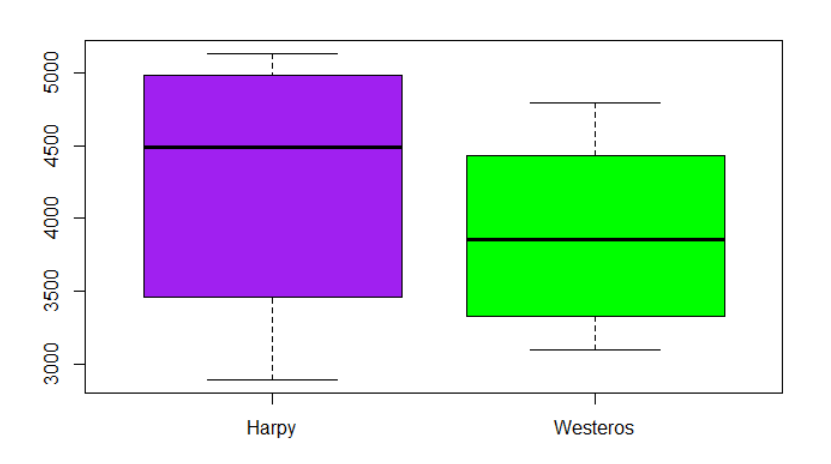
\includegraphics[width=100mm]{Graph.png}
		\caption{"Диаграммы размаха"}
		\label{Graph}
	\end{figure}
\end{frame}


\begin{frame}
\frametitle{Описание решения}
Далее, прогнозируем значения. Для этого найдём количество сломавшихся мечей относительно произведённых в долях единицы и отследим зависимость значений от каких-либо внешних факторов. Кривые значений ищем отдельно для каждой компании. В цикле находим максимальное и минимальное значение доли единицы количества сломавшихся мечей.
Усредняем полученные значения по всем кузнецам компании, анализируем полученные результаты значений обеих компаний.
\end{frame}

\begin{frame}{Описание решения}	
	\begin{figure}[h]
		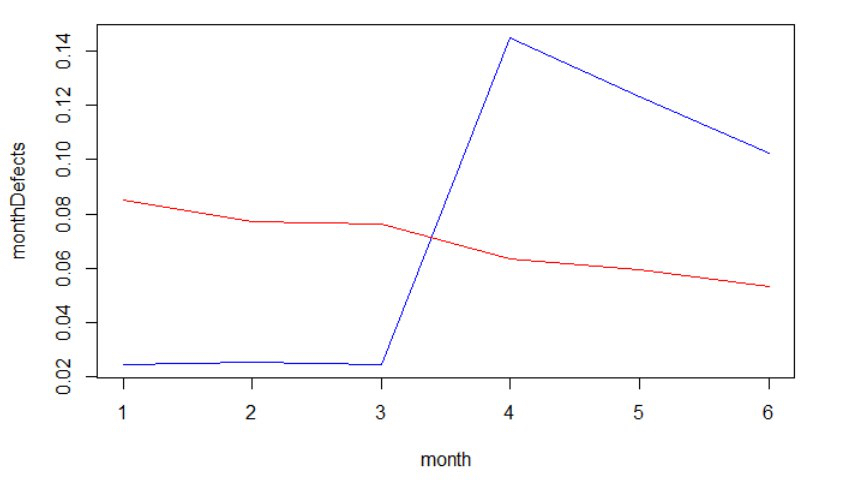
\includegraphics[width=100mm]{second.jpg}
		\caption{"Графики количества сломавшихся мечей"}
		\label{second}
	\end{figure}
\end{frame}

\begin{frame}
\frametitle{Анализ результатов}
Анализируем полученные после выполнения программы графики.\\
1 график: Разброс максимальных и минимальных значений количества целых мечей больше у компании Harpy \& Co, нежели у компании Westeros Inc.. Это означает, что у второй компании качество партий не так сильно отличается друг от друга, что показывает стабильность производства и является плюсом. Медиана количества целых мечей у компании Harpy \& Co больше, чем у компании  Westeros Inc.. Это означает, что в среднем качество мечей первой компании всё же выше, чем у второй.\\
\end{frame}

\begin{frame}
\frametitle{Анализ результатов}
2 график: Видно, что для у компании Westeros с третьего месяца происходит сильный рост количества сломавшихся мечей, что не зависит от какого-то конкретного кузнеца. Мечи компании Harpy ломаются равномерно в течение всего наблюдаемого времени.
\end{frame}

\begin{frame}
\frametitle{Вывод}
Далее по полученным анализам делаем вывод, с какой компанией следует сотрудничать.\\
Поскольку контракт будет заключаться на долговременный период (т.е. 11 месяцев), значение медианы и кривых поломки мечей имеет больший вес, чем разброс максимальных и минимальных значений. Следовательно, делаем вывод, основываясь на результатах анализа медианы и кривых поломки.\\
Таким образом, наиболее выгодно будет заключить контракт с компанией Harpy \& Co.
\end{frame}

\begin{frame}{Задание выполняли}
	\begin{itemize}
		{\small
		\item Пахомова Маргарита, студентка 411 группы. Написание программы
		\item Пантелеева Анастасия, студентка 411 группы. Написание Rnotebook и презентации
		\item Кулик Артем, студент 411 группы. Написание программы
		\item Чабан Олег, студент 412 группы. Написание презентации}
	\end{itemize}	

\end{frame}


\end{document}